\documentclass[a4paper,8pt]{beamer}
\usetheme{Madrid}
\usecolortheme{seahorse}
\usepackage[retainorgcmds]{IEEEtrantools}
\usepackage{graphicx}
\usepackage{physics}
\usepackage{bm,bbm}
\usepackage{tabularx,multirow,booktabs}
\usepackage{subcaption}
\usefonttheme{serif}
\title[Free energy]{Research update}
\date{\today}
\author{Sree Ganesh}
\institute[U of A]{Schwartz Group \\ University of Arizona}
\begin{document}
\maketitle
%
%------------------------------------------------------------------------------
% SLIDE 1
%------------------------------------------------------------------------------
%
%\begin{frame}
%\frametitle{Contents}
%\begin{itemize}
%  \item Introduction
%	\item Convergence tests
%	\item Hartree-Fock and the case of Conjugated acenes
%	\item Sodium clusters and inclusion of temperature effects
 %  \item Non-orbital-optimized RPA based polarizabilities 
%\end{itemize}
%\end{frame}
%------------------------------------------------------------------------------
%
%------------------------------------------------------------------------------
% SLIDE 6
%------------------------------------------------------------------------------
%
\begin{frame}
\frametitle{Free energies from TPS}
%For a given coordinate $\lambda$, the free energy profile along this coordinate ($A(\lambda)$) is given by
%\begin{equation}
%A(\lambda) = -k_BT\ln(P(\lambda)) \nonumber 
%\end{equation}
For an ensemble of unbiased trajectories 
the equilibrium probability distribution of the order parameter is  
\begin{equation}
P(\tilde{\lambda_i}) = \int d\vec{r}d\vec{p}\;\rho(\textbf{q})\sum^{\tau}_{j=1}\delta\left[\tilde{\lambda_i}-\lambda^j_i\right] \nonumber 
\end{equation}
\pause
The potential of mean force (PMF) can be expressed as 
\begin{equation}
\Phi_i(\lambda_i) = -k_BT\ln[P(\lambda_i)] + const. \nonumber 
\end{equation}
The free energy is calculated from the PMF as
\begin{equation}
exp(-\beta F) =\int^{\lambda_{\max}}_{\lambda_{min}} exp(-\beta\Phi(\lambda_i))d\lambda_i \nonumber 
\end{equation}
%where $\rho(\bf{q})$ is the equilibrium distribution function of the phase space configurations. \newline \pause
%$P(\tilde{\zeta})$ is often approximated as histograms.
\pause
The probability distribution function is often obtained as histograms.
\end{frame}
%

\begin{frame}
\frametitle{}
Protocol:
\begin{itemize}
\item Define order parameter window $\lambda_{i,min}<\lambda_i<\lambda_{i,max}$
\item Harvest dynamics trajectories using the TPS algorithm accepting them only if they visit 
 $\lambda_{i,min}<\lambda_i<\lambda_{i,max}$
 \item Use the ensemble of accepted trajectories to build the histogram for each interval (bin) 
 $P(\lambda_i)$
 \item Combine them to obtain $P(\lambda)$ by adjusting constants 
\end{itemize}
\pause
\begin{figure}
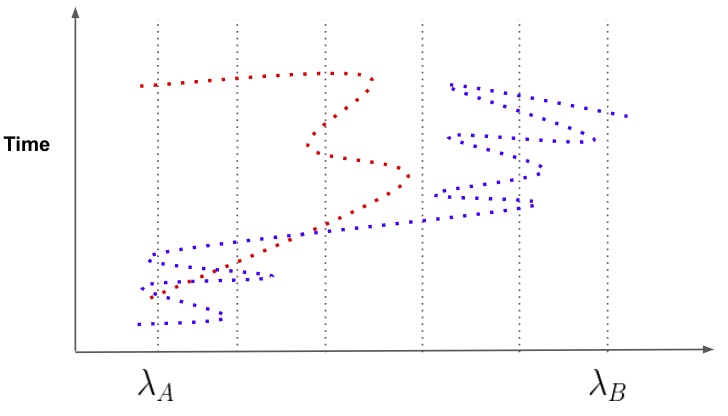
\includegraphics[scale=0.3]{bolas_tps_1.png}
\end{figure}
\end{frame}

\begin{frame}
\frametitle{Combining the probabilities in the individual windows}
Weighted histogram analysis method (WHAM).
\begin{equation}
P(\lambda) = \sum^{windows}_j w(\lambda_j)P(\lambda_j) \nonumber 
\end{equation}
The weights $w_j$ are chosen to minimize the statistical error of $P(\lambda)$
\begin{equation}
\frac{\partial^2\sigma(P(\lambda))}{w(\lambda_j)} = 0 \nonumber 
\end{equation}
such that $\sum_jw(\lambda_j)=0$.
Optimal weights are obtained by solving a set of coupled equations. 
\end{frame}

\end{document}
